\documentclass{standalone}
\usepackage{tikz, pgfplots, amssymb, amsmath, amsfonts}
\pgfplotsset{compat=1.18}
\usetikzlibrary {arrows.meta}
\newcommand{\vect}[1]{\boldsymbol{\mathbf{#1}}}
\begin{document}
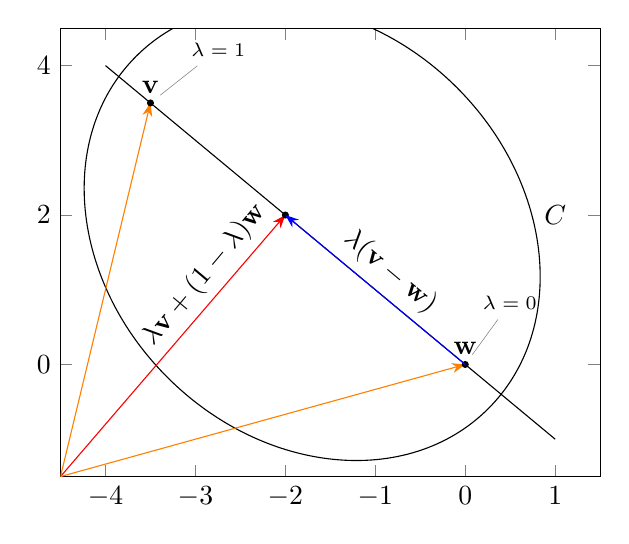
\begin{tikzpicture}
    \begin{axis}
    \draw[rotate=45,label={C}](-.75,-1)ellipse(74pt and 90pt);    
    \addplot[smooth, domain=-4:1]{-x};
    \draw[red,-Stealth](axis description cs:0,0)--(-2,2)coordinate(b)node[black,draw,circle, fill=black, inner sep=0.75pt]{}node[black,above left,rotate=50]{$\lambda\vect{v}+(1-\lambda)\vect{w}$}
    ;
    \draw[orange,-Stealth](axis description cs:0,0)--(0,0)coordinate(a)node[black,draw,circle, fill=black, inner sep=0.75pt]{}node[black, above]{$\vect{w}$}
    ;
    \draw[-Stealth,blue](a)--(b)node[midway, above,black,rotate=-40]{$\lambda(\vect{v}-\vect{w})$};
    \draw[orange,-Stealth](axis description cs:0,0)--(-3.5,3.5)coordinate(c)node[black,draw,circle, fill=black, inner sep=0.75pt]{}node[black, above]{$\vect{v}$}
    ;
    \draw(c)node[pin=50:{\scriptsize$\lambda=1$}]{};
    \draw(a)node[pin=80:{\scriptsize$\lambda=0$}]{};
    \draw(1,2)node{$C$};
    \end{axis}
\end{tikzpicture}
\end{document}